\section{Problema 2}
Se puede definir un límite de desviación estándar 2 en el error de estimación con cualquier estimador para el cual se pueda hallar una estimación razonable del error estándar.
\begin{enumerate}
\item  a) Explique por qué. Supóngase que $Y_{1}, Y_{2}, \ldots, Y_{n}$ representa una muestra aleatoria de una distribución de Poisson con media $\lambda$. Se conoce que $\operatorname{VAR}\left(Y_{i}\right)=\lambda$.
\begin{solution}
    Vamos a considerar el \textbf{Cuadro 3.4} del libro de texto:
    \begin{center}
        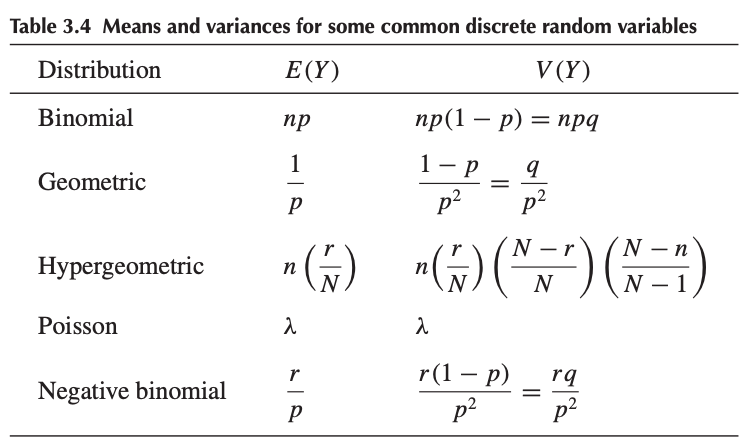
\includegraphics[scale=0.5]{Images/Problema2-1.png}
    \end{center}
    
    Además, el \textbf{Cuadro 1} del apéndice: 
    \begin{center}
        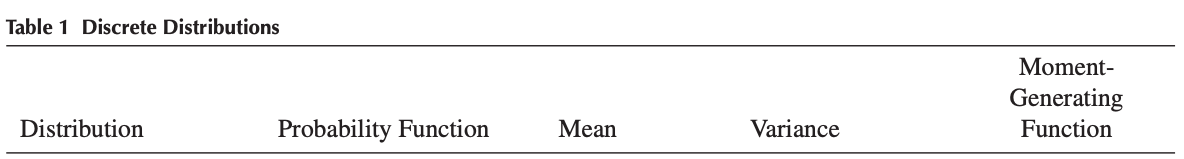
\includegraphics[scale=0.35]{Images/Problema2-2.png}
        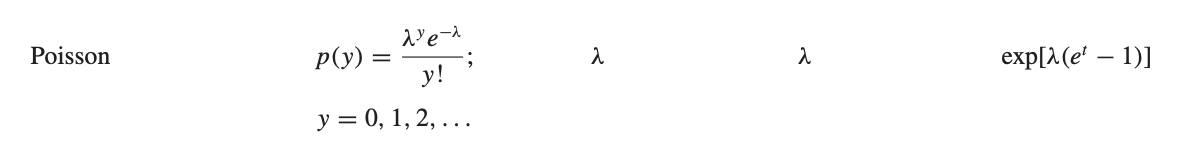
\includegraphics[scale=0.35]{Images/Problema2-3.png}
    \end{center}
    
    \linea
    
    Por definición se conoce que:
    \begin{gather}
        \operatorname{VAR}(Y) =E[Y(Y-1)]+E(Y) -[E(Y)]^2
    \end{gather}
    
    \linea 
    
    En donde $E(Y)$: 
    \begin{align*}
        E[Y] &= \sum_{y=0}^{\infty}\frac{y\lambda^ye^{-\lambda}}{y!} 
        \intertext{En donde el primer término ($y=0$) es 0, por lo cual: }
             &= \sum_{y=1}^{\infty}\frac{y\lambda^ye^{-\lambda}}{y!}=\lambda\sum_{y=1}^{\infty}\frac{\lambda^{y-1}e^{-\lambda}}{(y-1)!}
        \intertext{Se propone un cambio de variables $z= y-1$:}
             &= \lambda\sum_{z=0}^{\infty}\frac{\lambda^ze^{-\lambda}}{z!}
        \intertext{Nótese que $p(z)=\frac{\lambda^ze^{-\lambda}}{z!}$ es la función de probabilidad para una variable aleatoria de Poisson; entonces $\sum_{z=0}^{\infty}p(z)=1$, por lo tanto:}
             &= \lambda
    \end{align*}
    
    \linea 
    
    En donde $E[Y(Y-1)]$: 
    
    
    
    \begin{align*}
        E[Y(Y-1)] &= \sum_{y=0}^{\infty}\frac{y(y-1)\lambda^ye^{-\lambda}}{y!}
        \intertext{En donde el primer término  y segundo término ($y=0,1$) son 0, por lo cual:}
                 &=\sum_{y=2}^{\infty}\frac{y(y-1)\lambda^ye^{-\lambda}}{y!}=\lambda^2 \sum_{y=2}^{\infty}\frac{\lambda^{y-2}e^{-\lambda}}{(y-2)!}
        \intertext{Se propone un cambio de variables $z= y-2$:}
        &= \lambda^2\sum_{z=-2}^{\infty}\frac{\lambda^{z}e^{-\lambda}}{z!}
         \intertext{Nótese que $p(z)=\frac{\lambda^ze^{-\lambda}}{z!}$ es la función de probabilidad para una variable aleatoria de Poisson; entonces $\sum_{z=0}^{\infty}p(z)=1$, por lo tanto:}
             &= \lambda^2
    \end{align*}
    
     \linea 
    
    Regresando a (1), tenemos: 
    \begin{align}
        \operatorname{VAR}(Y) &=E[Y(Y-1)]+E(Y) -[E(Y)]^2\\
        &= \lambda^2 +\lambda -\lambda^2\\
        &= \lambda
   \end{align}
   
   \linea 
   
   Regresando al problema original, se indica que $Y_1,Y_2,...,Y_n$ son variables aleatorias que representan una muestra aleatoria de una distribución de Poisson y con media $\lambda$. Ahora bien, basándonos en toda la argumentación anterior, la explicación de que  $\operatorname{VAR}(Y_i)=\lambda$ es que $i$ es un contador y cada una de las variables aleatorias $Y_i$ son iguales a $\lambda$. Análogamente, es la misma argumentación para $E(Y_i)=\lambda$.

    \end{solution}
\item  b) Calcule $\mathrm{E}(\overline{Y})$ y $\operatorname{VAR}(\overline{Y})$.

\begin{tcolorbox}[colback=gray!15,colframe=black!1!black,title=Teorema 5.12]
Sea $Y_{1}, Y_{2}, \ldots, Y_{n}$ y $X_{1}, X_{2}, \ldots, X_{m}$ variable aleatorias con $E\left(Y_{i}\right)=\mu_{i}$ y $E\left(X_{j}\right)=\xi_{j}$. Se define
$$
U_{1}=\sum_{i=1}^{n} a_{i} Y_{i} \quad \text { and } \quad U_{2}=\sum_{j=1}^{m} b_{j} X_{j}
$$
para constantes $a_{1}, a_{2}, \ldots, a_{n}$ and $b_{1}, b_{2}, \ldots, b_{m} .$ Entonces, lo siguiente se mantiene: 
\begin{enumerate}
    \item $E\left(U_{1}\right)=\sum_{i=1}^{n} a_{i} \mu_{i} .$
    \item  $V\left(U_{1}\right)=\sum_{i=1}^{n} a_{i}^{2} V\left(Y_{i}\right)+2 \sum \sum_{1 \leq i<j \leq n} a_{i} a_{j} \operatorname{Cov}\left(Y_{i}, Y_{j}\right)$, donde
la doble suma está sobre todos los pares $(i, j)$ con $i<j$.
    \item $
\operatorname{Cov}\left(U_{1}, U_{2}\right)=\sum_{i=1}^{n} \sum_{j=1}^{m} a_{i} b_{j} \operatorname{Cov}\left(Y_{i}, X_{j}\right) .
$
\end{enumerate}


\end{tcolorbox}
\begin{solution}
    Sabemos que $\overline{Y}$ hace referencia a la media muestral: 
    \begin{gather*}
        \overline{Y}= \frac{1}{n}\sum_{i=1}^{n}Y_i
    \end{gather*}
    
    \linea 
    
    El valor esperado (aplicando las propiedades previamente conocidas): 
    
    \begin{align*}
        E(\overline{Y}) &= E\left(\frac{1}{n}\sum_{i=1}^{n}Y_i\right)  = \frac{1}{n}E\left(\sum_{i=1}^{n}Y_i\right)\\
        &= \frac{1}{n}E\left(Y_1+Y_2+Y_3+...+Y_n\right)\\
        &=\frac{1}{n}\left[E(Y_1)+E(Y_2)+E(Y_3)+...+E(Y_n)\right]\\
        &= \frac{1}{n}\left[\lambda+\lambda+\lambda+...+\lambda\right]\\
        &= \frac{1}{n}\left[n\lambda\right]\\
        &= \lambda
    \end{align*}
    
    \linea 
    
    La varianza (basándose en el \textbf{teorema 5,12}) : 
    
    \begin{align*}
        \operatorname{VAR}(\overline{Y}) &=  \sum_{i=1}^{n} \left(\frac{1}{n}\right)^{2} \operatorname{VAR}\left(Y_{i}\right)+2 \sum \sum_{1 \leq i<j \leq n} \left(\frac{1}{n}\right)^{2} \left(\frac{1}{n}\right)^{2} \operatorname{Cov}\left(Y_{i}, Y_{j}\right) \\
        &= \sum_{i=1}^{n}\left(\frac{1}{n}\right)^2\operatorname{VAR}(Y_i) =\left(\frac{1}{n}\right)^2\sum_{i=1}^{n}\operatorname{VAR}(Y_i) \\
        &= \left(\frac{1}{n}\right)^2n\lambda\\
        &= \frac{\lambda}{n}
    \end{align*}
    
    \end{solution}
\item c) ¿Cómo emplearía $Y_{1}, Y_{2}, \ldots, Y_{n}$ para estimar $\lambda ?$
\begin{solution}
    Se conoce ampliamente que $\overline{Y}$ es un estimador de una muestra de variables aleatorias $Y_1,Y_2,Y_3,\cdots, Y_n$. Por lo cual: 
    $$\hat{\lambda}=\overline{Y}$$
    \end{solution}
\item d) ¿Cómo estimaría el error estándar de su estimador propuesto en c)? (Valor 25 puntos).
\begin{solution}
    Esto es bastante sencillo, ya que sabemos que: 
    $$\operatorname{VAR}(\overline{Y})=\frac{\lambda}{n}$$
que es estimado por medio de: 
$$\frac{\hat{\lambda}}{n}=\frac{\overline{Y}}{n}$$
Por lo tanto, el error estándar del estimador es estimado por: 

$$\sqrt{\frac{\overline{Y}}{n}}$$
    \end{solution}
\end{enumerate}
